%!TEX root=../GaugeCNNTheory.tex


\subsection{Isometry actions and induced gauge transformations}
\label{sec:isometries_local}


Until now our discussion focused exclusively on the local gauge symmetries in the coordinatization of tangent spaces.
A manifold might, however, come with non-trivial symmetries itself, which are in the case of a Riemannian manifold~$M$ forming its \emph{isometry group} $\IsomM$.
This section discusses isometries and their action on manifolds, tangent vectors, reference frames and feature fields in a nutshell, summarizing results which are more rigorously derived in Section~\ref{sec:isom_background}.
We will thereby highlight the equivalence of \emph{active} isometry actions and their \emph{passive} interpretation in terms of isometry induced gauge transformations.
This equivalence will later on allow us to describe the isometry equivariance of $\GM$-convolutions.


Isometries are defined as the symmetries of Riemannian manifolds, that is, those maps (diffeomorphisms)
\begin{align}
    \phi: M \to M,
\end{align}
that preserve the metric and thus distances on~$M$.
The set of all isometries of a Riemannian manifold~$M$ forms its isometry group, which we denote as $\IsomM$.
For instance, the Euclidean group~$\E{d}$ is the isometry group of Euclidean spaces~$\Euc_d$.
It consists of translations, rotations and reflections, all of which preserve the standard metric of~$\Euc_d$.
The isometry group of the $2$-sphere $S^2$ is given by the orthogonal group $\O3$, consisting of rotations and reflections.
Fig.~\ref{fig:pushforward_vector_components} shows an egg-shaped manifold, whose isometries are rotations and reflections in $\O2$ around the vertical axis.


\begin{SCfigure}[1.8]
    \centering
    \hspace{.5ex}
    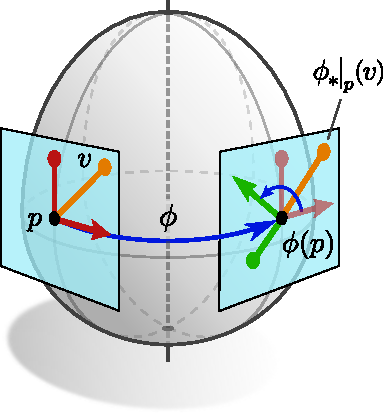
\includegraphics[width=.35\textwidth]{figures/isometry_egg_tangent_vector_gauge_trafo.pdf}
    \caption[]{\small
        Visualization of the coordinate free pushforward of tangent vectors and its coordinate expression relative to given reference frames at the source and target location.
        The coordinate free pushforward ${\phi_*|_p: \TpM \to \TphipM}$ moves tangent vectors $\ v \!\in\! \TpM\ $ to $\ \phi_*|_p(v) \!\in\! \TphipM\,$ (orange).
        Let $\psi_p^{\widetilde{A}}$ be the gauge at $p$ that corresponds to the red reference frame and $\psi_{\phi(p)}^A$ the gauge at $\phi(p)$ that corresponds to the green reference frame.
        They explain the vectors before and after the pushforward by numerical coefficients $\psi_p^{\widetilde{A}}(v) = (1,1)^\top$ and $\psi_{\phi(p)}^A \big( \phi_*|_p(v) \big) = \big(0,-\sqrt{2}\big)^\top$.
        This transformation of vector coefficients is described by the isometry induced gauge transformation $g_\phi^{A\widetilde{A}}(p) \in \GL{d}$, that is,
        $\psi_{\phi(p)}^A \big( \phi_*|_p(v) \big) = g_\phi^{A\widetilde{A}}(p) \cdot \psi_p^{\widetilde{A}}(v)$.
        The coefficients of feature vectors transform analogously according to $\rho\big( g_\phi^{A\widetilde{A}}(p) \big)$ if $g_\phi^{A\widetilde{A}}(p) \in G$.
        \\[1ex]
        }
    \label{fig:pushforward_vector_components}
\end{SCfigure}





\subsubsection{Pushforward of tangent vectors}

Any isometry $\phi \in \IsomM$ acts via its \emph{pushforward} (or differential)
\begin{align}
    \phi_{*}|_p:\, \TpM \to \TphipM \,,
\end{align}
naturally on tangent vectors.
As visualized in Fig.~\ref{fig:intro_gauge_isom_induction} (middle), the pushforward can intuitively be thought of as carrying tangent vectors along with the action of the isometry on the underlying manifold~$M$.
A formal definition of the pushforward on $\TM$ is given in Appendix~\ref{apx:differentials_gradients_jacobians}, however, the given intuition is sufficient for our purpose.
Since the pushforward is a coordinate free, linear map between tangent spaces, its action is in coordinates represented by some $d\times d$ matrix.
Assuming gauges $\psi_p^{\widetilde{A}}$ and $\psi_{\phi(p)}^A$ at the source and target location, respectively, this matrix is given by
\begin{align}\label{eq:isom_induced_gauge_trafo_24}
    g_\phi^{A\widetilde{A}}(p)\ :=\ \psi_{\phi(p)}^A \circ \phi_*|_p \circ \big( \psi_p^{\widetilde{A}} \mkern1mu\big)^{-1} \ \ \in\, \GL{d} \,.
\end{align}
It explains the transformation from the numerical coefficients of an original vector $v\in\TpM$ in the source gauge and its pushforward $\phi_*|_p(v) \in\TphipM$ in the target gauge, that is,
$\psi_{\phi(p)}^A \big( \phi_*|_p (v) \big) = g_\phi^{A\widetilde{A}}(p) \cdot \psi_p^{\widetilde{A}}(v)$.
The commutative diagram
\begin{equation}
\begin{tikzcd}[column sep=54pt, row sep=28pt, font=\normalsize]
    \R^d
        \arrow[dd, "g_p^{\widetilde{B}\widetilde{A}}\cdot\ "']
        \arrow[rrr, "g_\phi^{A\widetilde{A}}(p)\cdot"]
    & &[-1ex] &
    \R^d
        \arrow[dd, "\ g_{\phi(p)}^{BA}\cdot"]
    \\
    &
    \TpM
        \arrow[ul, "\psi_p^{\widetilde{A}}"]
        \arrow[dl, "\psi_p^{\widetilde{B}}"']
        \arrow[r, "\phi_*|_p"]
    &
    \TphipM
        \arrow[ur, "\psi_{\phi(p)}^A"']
        \arrow[dr, "\psi_{\phi(p)}^B"]
    \\
    \R^d
        \arrow[rrr, "g_\phi^{B\widetilde{B}}(p)\cdot"']
    & & &
    \R^d
\end{tikzcd}
\quad,
\end{equation}
which is conceptually similar to that in Eq.~\eqref{cd:transporter_trivialization}, visualizes the definition of the tangent vector pushforward's coordinate expression.
It furthermore implies that the gauge transformations between different coordinatizations are given by
\begin{align}
    g_\phi^{B\widetilde{B}}
    \ =\ g_{\phi(p)}^{BA} \; g_\phi^{A\widetilde{A}} \mkern1mu \big(g_p^{\widetilde{B}\widetilde{A}} \mkern1mu\big)^{-1} \,,
\end{align}
which is the conceptual analog to Eq.~\eqref{eq:transporter_gauge_trafo}.










\subsubsection{Pushforward of reference frames and symmetries of the \textit{G}-structure}

Since reference frames are just $d$-tuples of linearly independent frame vectors, the pushforward of tangent vectors induces a pushforward of reference frames by \emph{pushing the individual frame axes forward}.
Specifically, the pushforward of a frame $[e_i]_{i=1}^d$ at~$p$ is defined as the frame $\big[ \phi_*|_p (e_i) \big]_{i=1}^d$ at~$\phi(p)$.


This pushforward of frames is always well defined, however, it might not be compatible with the $G$-structure, that is, there is in general no guarantee that frames in $\GM$ remain in $\GM$ when being pushed forward.
Take for instance the $\{e\}$-structure in Fig.~\ref{fig:intro_invariant_kernel_fields_plane} (top left), which is preserved by horizontal translations but not by vertical translations or any other isometry of~$\R^2$.
Similarly, the $\Flip$-structure in Fig.~\ref{fig:intro_invariant_kernel_fields_plane} (bottom left) is preserved by translations and horizontal reflections, but not by rotations.
We consider therefore the subgroup
\begin{align}\label{eq:IsomGM_def_24}
    \IsomGM\ :=\ \pig\{ \phi \in \IsomM \ \pig|\ 
    \big[\phi_*(e_i)\big]_{i=1}^d \in \GM \quad \forall\ [e_i]_{i=1}^d \in \GM \pig\} \,\ \leq\ \IsomM
\end{align}
of \emph{isometries which are symmetries of the $G$-structure}, i.e. which are guaranteed to map any frame in~$\GM$ to another frame that is also contained in~$\GM$.%
\footnote{
    More formally stated, such isometries are (or induce) \emph{principal bundle automorphisms} of the $G$-structure.
}
Note that $\IsomGM$ depends in general on the specific choice of $G$-structure $\GM$, not only on the structure group~$G$.
For the special case that $G\geq\O{d}$, it is guaranteed that $\IsomGM=\IsomM$ coincide since isometries are guaranteed to map orthonormal frames to orthonormal frames.
We are interested in the subgroup $\IsomGM$ since only those isometries will induce a well defined pushforward of $\GM$-coordinate independent feature vectors, as discussed further in the following section.


Before proceeding to the isometry action on feature vectors, we discuss what we call \emph{isometry induced gauge transformations}.
For this purpose, let $\big[e_i^{\widetilde{A}} \big]_{i=1}^d$ be that frame at~$p$ that corresponds to some source gauge $\psi_p^{\widetilde{A}}$ and let $\big[e_i^A \big]_{i=1}^d$ be that frame at $\phi(p)$ that corresponds to some target gauge $\psi_{\phi(p)}^A$, as shown in Fig.~\ref{fig:pushforward_vector_components} in red (left) and green (right), respectively.
The pushforward $\big[\phi_*|_p( e_i^{\widetilde{A}}) \big]_{i=1}^d$ of the source frame from $p$ to $\phi(p)$ (translucent red, right) does in general not coincide with the target frame.
However, as proven in Section~\ref{sec:isom_coordinatization}, the two frames are related by the isometry induced gauge transformation
\begin{align}
    \pig[\phi_*|_p( e_i^{\widetilde{A}}) \pig] \raisebox{-2.5pt}{$\rule{0pt}{12pt}_{i=1}^d$}
    \ =\ \big[e_i^A \big]_{i=1}^d \lhd g_\phi^{A\widetilde{A}}(p) \,,
\end{align}
where $g_\phi^{A\widetilde{A}}(p)$ is the group element from Eq.~\eqref{eq:isom_induced_gauge_trafo_24} and $\lhd$ is the right action from Eq.~\eqref{eq:right_action_mapsto}.
The term ``isometry induced gauge transformation'' makes in so far sense that the geometries around $p$ and $\phi(p)$ are indistinguishable since $\phi$ is an isometry, i.e. a symmetry of~$M$.
Identifying the two points with each other, one can therefore reinterpret the \emph{active} action of $\phi$ on a geometric quantity as a \emph{passive} gauge transformation, i.e. an induced change from the source to the target frame.


Theorem~\ref{thm:isom_GM_in_coords} in Section~\ref{sec:isom_background} asserts that $G$-structure preserving isometries in $\IsomGM$ and $G$-valued induced gauge transformations imply each other, that is,
\begin{align}\label{eq:IsomGM_coord_in_G_24}
    \phi \in \IsomGM \quad \Longleftrightarrow \quad g_\phi^{A\widetilde{A}}(p) \in G\ \ \ \forall\ p \mkern-1mu\in\mkern-2mu M
\end{align}
holds for arbitrary gauges $\psi_p^{\widetilde{A}}$ and $\psi_{\phi(p)}^A$ of the $G$-atlas.
The reader should verify these claims at our examples in Fig.~\ref{fig:intro_invariant_kernel_fields_plane}.






\subsubsection{Pushforward of feature vectors}

If (and only if) an isometry is a symmetry of the $G$-structure, it gives rise to a \emph{pushforward of feature vectors}.
Intuitively, this pushforward moves feature vectors from points $p$ to $\phi(p)$.
When being expressed relative to the two reference frames at $p$ and $\phi(p)$, it is given by the induced gauge transformation
\begin{align}
    \rho\big( g_\phi^{A\widetilde{A}}(p) \big) \,.
\end{align}
Note that this transformation is well defined for any $\phi \in \IsomGM$, since the induced gauge transformations $g_\phi^{A\widetilde{A}}(p)$ will in this case take values in~$G$ and $\rho$ is a $G$-representation.
In contrast, if $\phi$ is not a symmetry of the $G$-structure, it is \emph{impossible} to define a corresponding feature vector pushforward.
This statement relates to the fact that the features of conventional CNNs have no specified transformation behavior under rotations or reflections in the Euclidean group~$\E{d}$.


The pushforward of individual feature vectors implies an action on the whole feature field $f$, which we denote by $\phi \rhd f$.
Relative to coordinates, this action is expressed as
\begin{align}\label{eq:feature_field_trafo_in_coords}
    \big[\phi \rhd f\big]^A(\phi(p)) \ =\ \rho\big( g_\phi^{A\widetilde{A}}(p)\big)\, f^{\widetilde{A}}(p) \,.
\end{align}
We will later prove that coordinate independent CNNs are equivariant w.r.t. the action of isometries in $\IsomGM$ on feature fields; see Fig.~\ref{fig:lizard_conv_egg}.
This property relies on the fact that the active isometry action on feature fields can by Eq.~\eqref{eq:feature_field_trafo_in_coords} be understood as a mere passive gauge transformation of feature vector coefficients.
